% Options for packages loaded elsewhere
\PassOptionsToPackage{unicode}{hyperref}
\PassOptionsToPackage{hyphens}{url}
%
\documentclass[
]{book}
\usepackage{lmodern}
\usepackage{amssymb,amsmath}
\usepackage{ifxetex,ifluatex}
\ifnum 0\ifxetex 1\fi\ifluatex 1\fi=0 % if pdftex
  \usepackage[T1]{fontenc}
  \usepackage[utf8]{inputenc}
  \usepackage{textcomp} % provide euro and other symbols
\else % if luatex or xetex
  \usepackage{unicode-math}
  \defaultfontfeatures{Scale=MatchLowercase}
  \defaultfontfeatures[\rmfamily]{Ligatures=TeX,Scale=1}
\fi
% Use upquote if available, for straight quotes in verbatim environments
\IfFileExists{upquote.sty}{\usepackage{upquote}}{}
\IfFileExists{microtype.sty}{% use microtype if available
  \usepackage[]{microtype}
  \UseMicrotypeSet[protrusion]{basicmath} % disable protrusion for tt fonts
}{}
\makeatletter
\@ifundefined{KOMAClassName}{% if non-KOMA class
  \IfFileExists{parskip.sty}{%
    \usepackage{parskip}
  }{% else
    \setlength{\parindent}{0pt}
    \setlength{\parskip}{6pt plus 2pt minus 1pt}}
}{% if KOMA class
  \KOMAoptions{parskip=half}}
\makeatother
\usepackage{xcolor}
\IfFileExists{xurl.sty}{\usepackage{xurl}}{} % add URL line breaks if available
\IfFileExists{bookmark.sty}{\usepackage{bookmark}}{\usepackage{hyperref}}
\hypersetup{
  hidelinks,
  pdfcreator={LaTeX via pandoc}}
\urlstyle{same} % disable monospaced font for URLs
\usepackage{longtable,booktabs}
% Correct order of tables after \paragraph or \subparagraph
\usepackage{etoolbox}
\makeatletter
\patchcmd\longtable{\par}{\if@noskipsec\mbox{}\fi\par}{}{}
\makeatother
% Allow footnotes in longtable head/foot
\IfFileExists{footnotehyper.sty}{\usepackage{footnotehyper}}{\usepackage{footnote}}
\makesavenoteenv{longtable}
\usepackage{graphicx,grffile}
\makeatletter
\def\maxwidth{\ifdim\Gin@nat@width>\linewidth\linewidth\else\Gin@nat@width\fi}
\def\maxheight{\ifdim\Gin@nat@height>\textheight\textheight\else\Gin@nat@height\fi}
\makeatother
% Scale images if necessary, so that they will not overflow the page
% margins by default, and it is still possible to overwrite the defaults
% using explicit options in \includegraphics[width, height, ...]{}
\setkeys{Gin}{width=\maxwidth,height=\maxheight,keepaspectratio}
% Set default figure placement to htbp
\makeatletter
\def\fps@figure{htbp}
\makeatother
\setlength{\emergencystretch}{3em} % prevent overfull lines
\providecommand{\tightlist}{%
  \setlength{\itemsep}{0pt}\setlength{\parskip}{0pt}}
\setcounter{secnumdepth}{5}
% Starts each section (##) on a new page
% https://tex.stackexchange.com/questions/9497/start-new-page-with-each-section
\let\stdsection\section
\renewcommand\section{\clearpage\stdsection}

% Needs latex_engine: xelatex in _output.yml. Doesn't work yet.
\usepackage{fontspec}

\author{}
\date{\vspace{-2.5em}}

\begin{document}

%\newgeometry{tmargin=1.5cm,lmargin=2.5cm,rmargin=2.5cm,bmargin=0.5cm} %verbose

\begin{titlepage}
\begin{center}
  

\end{center}
\vspace{1.5cm}
\begin{center}

{\LARGE Songs}

\end{center}
 \vspace{1cm}

\begin{figure}[htbp]
  \centering
  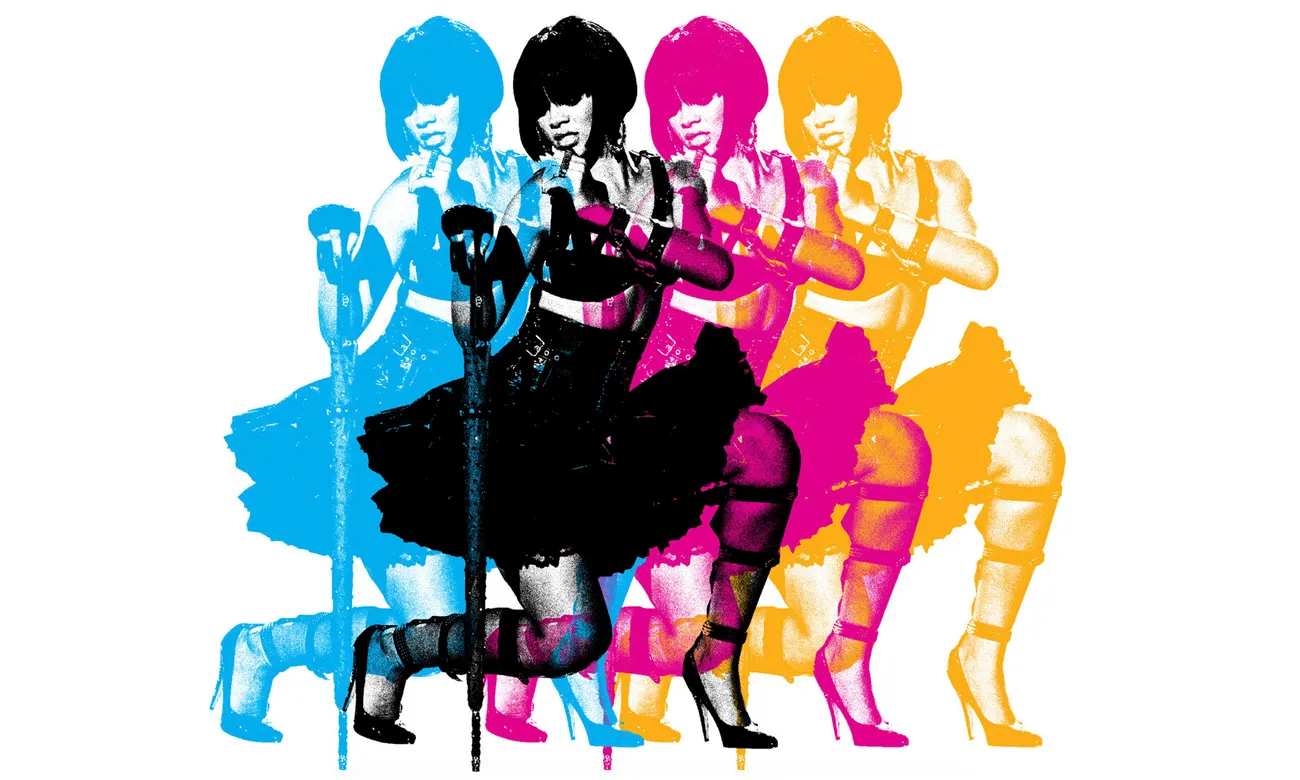
\includegraphics[width=1\textwidth]{misc/title.png}
  \label{titelbild}
\end{figure}

\begin{center}
\textbf{}


\end{center} 

\vspace{1.0cm}


\end{titlepage}
%\restoregeometry

{
\setcounter{tocdepth}{1}
\tableofcontents
}
A collection of hand picked songs. This book is hosted as an online version on \url{https://ratnanil.github.io/Songs/} and includes pdf / epub versions (click on the download symbol). Edits and feedback can be made via the \href{https://github.com/ratnanil/songs}{github repo}. The current version was rendered on 2020-12-12 17:21:13.

\hypertarget{selected-songs}{%
\chapter{Selected Songs}\label{selected-songs}}

\hypertarget{dance-me-to-the-end-of-love---leonard-cohen}{%
\section{Dance me to the end of Love - Leonard Cohen}\label{dance-me-to-the-end-of-love---leonard-cohen}}

\begin{verbatim}

[Am]                          [Em]
Dance me to your beauty with a burning violin
[Am]                               [Em]
Dance me through the panic 'til I'm gathered safely in
[Am]                            [Em]
Lift me like an olive branch and be my homeward dove
[B7]                [Em]
Dance me to the end of love
[B7]                [Em]
Dance me to the end of love

Oh let me see your beauty when the witnesses are gone 
Let me feel you moving like they do in Babylon 
Show me slowly what I only know the limits of 
Dance me to the end of love 
Dance me to the end of love 

Dance me to the wedding now, dance me on and on 
Dance me very tenderly and dance me very long 
We're both of us beneath our love, we're both of us above 
Dance me to the end of love 
Dance me to the end of love

Dance me to your beauty with a burning violin 
Dance me through the panic till I'm gathered safely in 
Touch me with your naked hand or touch me with your glove 
Dance me to the end of love (3x)

{comment: play intro again}
\end{verbatim}

\end{document}
